\section{Introduction}

% dialogue -> fairness in dialogues => dialogue understanding tasks
%Dialogues as the most natural way for information exchanges has gained great attention and its research directions can be divided into two categories. One is open-ended dialogue systems~\cite{gu2021dialogbert,xu2021learning} which aims at generating or selecting appropriate responses to fulfill the users' needs. The other is dialogue understanding tasks which helps to quickly digest information and returns the expected output given the whole dialogue. 

%With the prosperous of fine-tuning with pre-trained language models, dramatic improvements have achieved on a range of dialogue tasks, pushing their implementation in practice. 
The safety and fairness issue of text generations from 
dialogue-related models is a crucial concern when implementing 
generation results from dialogue models in real applications. 
Previous work mainly focuses on responses from open-ended dialogue systems~\cite{xu2020recipes, henderson2018ethical}, such as offensive contents~\cite{baheti2021just}, gender bias~\cite{liu2020does,dinan2020queens} and other discriminated behavior~\cite{sheng2021revealing,smith2021hi}. For close-form dialogue 
understanding and generation tasks, where the whole dialogue is provided and the 
output shouldn't go beyond the dialogue, 
the fairness issue is still unexplored.

% leaving the fairness of close-style dialogue understanding tasks unexplored.

\begin{figure}[th]
	\centering
	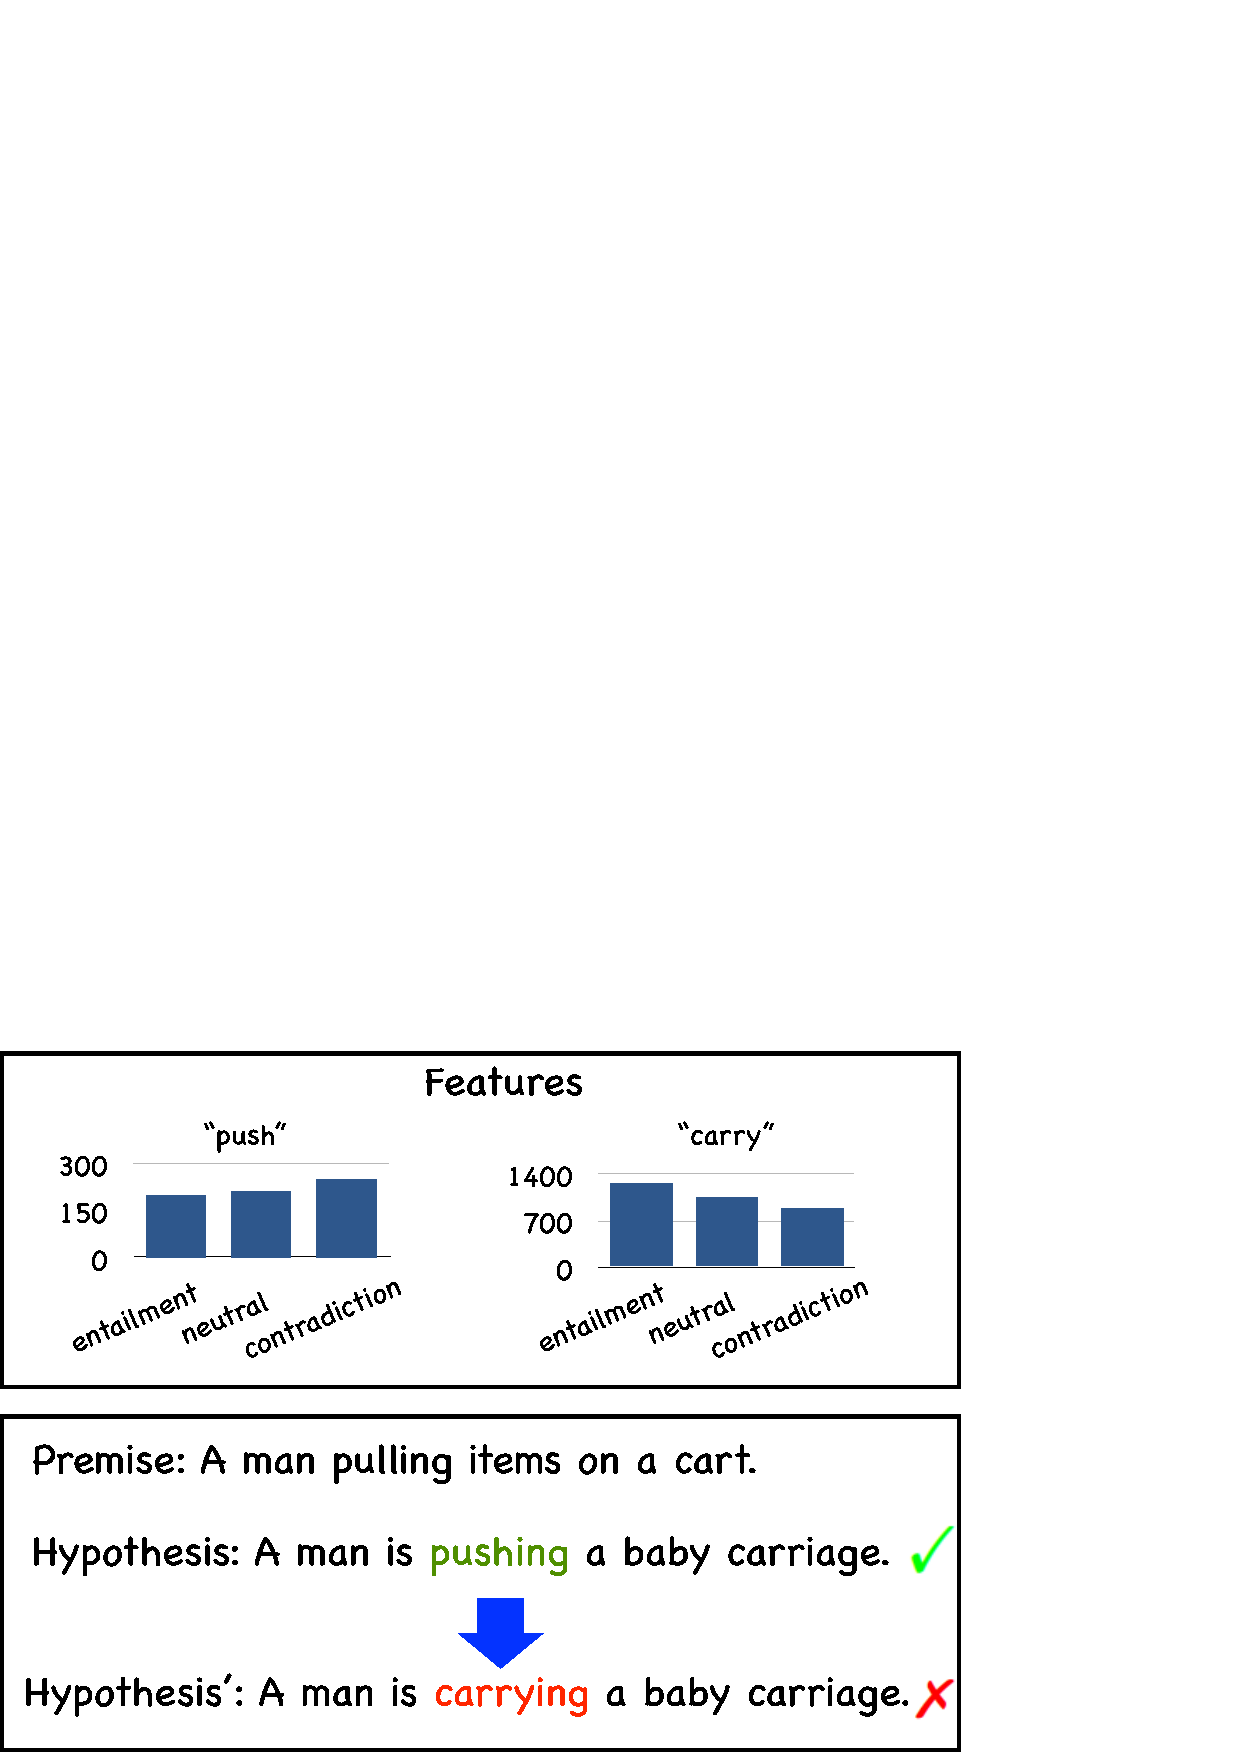
\includegraphics[width=0.95\columnwidth]{example.pdf}
	\caption{Two instances of an example from the SAMSum dataset, each
with a different set of names. Two different summaries are generated by BART. 
Different Colors indicate different speakers. 
In the generated summaries, \textit{incorrect contents} are italicized, 
while \underline{divergent contents} are underlined.}
	\label{fig:example}
\end{figure}

% dialogue understanding tasks, characteristics  with example
%Representative dialogue understanding tasks includes dialogue summarization~\cite{lin2022other,zhong2022dialoglm}, reading comprehension~\cite{sun2019dream,li2020molweni}, and etc. 
In these tasks, such as dialogue summarization~\cite{lin2022other,zhong2022dialoglm}, the input dialogues are self-contained, and the names of the speakers
should not carry any connotation from outside of the dialogue. Therefore,
changing the speaker names consistently in a dialogue should not affect the 
meanings of the dialogue.
Taking the dialogues from dialogue summarization task in 
Figure~\ref{fig:example} as an example, the utterances in dialogue-1 and
dialogue-2 are identical except for the speakers' names. 
The summaries for the two dialogues are expected to be the same modulo 
the speaker names. 
%In conclusion, speaker name insensitivity is an inherent and obvious characteristic of dialogue understanding.

% robustness of language model
Unfortunately, models nowadays, following the pretrain-finetune paradigm, 
are sensitive to trivial changes, which has been verified in other works. 
In relation extraction, spurious correlations between entity mentions and 
relations lead to entity bias. 
Some work~\cite{zhang2018graph,zhang-etal-2017-position} proposes to 
prevent it by masking entities during fine-tuning. 
\citet{wang-etal-2022-rely} debiases the models by removing the 
counterfactual predictions based on causal inference. 
Other similar work includes the analysis of robustness by entity 
renaming for machine reading comprehension models on narrative 
texts~\cite{yan2022robustness} and name biases in machine translation 
with inflected languages~\cite{wang2022measuring}, like German. 


% sensitivity of PrLMs in dialogue understanding tasks
Obviously, dialogue understanding models are sensitive to speaker names 
according to Figure~\ref{fig:example} as well. Incorrect content, 
``Betsy don't want to go'', is generated with the first group of speakers, 
while not with the other. The model also tends to focus on different viewpoints 
with different speaker names, such as ``don't want to go'' and 
``doesn't like them''.  Such uneven performances create unfairness among 
different name uses. The model may also catch the latent properties 
in names~\cite{romanov2019s} and lead to discrimination against 
specific groups of people, raising the importance of research on the fairness of dialogue models by reducing the sensitivity of speaker names.
%Different from named entities, 
%\KZ{Don't understand this: 
%speakers in these tasks are more isolated 
%from the dialogue contents and have closer connections to users in real applications}, 


Previous work has also mentioned this problem. Different data pre-processing approaches are adopted during the construction of datasets to avoid using speaker names, such as ``A'' or ``B'' in \citet{li2017dailydialog}. \citet{khalifa2021bag} replace speaker names with more common and frequent names that the model may have seen during pre-training. Data augmentation by changing speaker names is adopted by \citet{liu2021controllable}.
However, all of these works only attempted to attack this problem 
subjectively, without quantitive analysis and fair comparisons.

% approach classification / our approach
In this work, we systematically analyze speaker name sensitivity in dialogue 
understanding tasks. We formulate the problem and divide the approaches 
into offline ones and online ones. The model needs fine-tuning for both 
approaches. The difference is that online approaches require additional 
data pre-processing and post-processing steps during inference, 
while offline approaches don't. 
Besides, we further propose a novel Insensitivity Loss, helping to reduce attention distances of the same dialogue with different speaker names for transformer-based models during fine-tuning. This loss can be used in both online approaches and offline approaches.
Results on dialogue summarization and question generation show that the
online approach which replaces names with frequent ones achieves the best generation performance, and coupled with data augmentation, it gives the provides
the most speaker name fairness among all baselines.
Our approach with Insensitivity Loss can further reduce the sensitivity in both kinds of approaches and get better results on task-specific metrics, achieving state-of-the-art performance.
%\KZ{I'm a little confused reading the above two sentences. Which one is better,
%the freq or our ins loss?}

% contributions
In summary, our contributions are as follows:
\begin{itemize}
	\item We are the first to investigate the speaker name fairness 
in close-form dialogue understanding and generation tasks (Sec.~\ref{sec:problem}). % and quantify the performance sensitivity for further analysis
	\item We introduce Insensitivity Loss as an auxiliary training objective for reducing sensitivity during fine-tuning (Sec.~\ref{sec:approach}).
	\item Extensive experiments on different tasks provide a comprehensive benchmark with quantitative analysis on speaker name sensitivity and show 
the favorable performances of our approach
%stronger overall performance with lower speaker name sensitivity 
(Sec.~\ref{sec:results}).
\end{itemize}
